\begin{frame}
	\myheading{Module 21.2: Variational Autoencoders: The Neural Network Perspective}
\end{frame}

\begin{frame}
	\begin{columns}
		\column{0.4\textwidth}
		\begin{overlayarea}{\textwidth}{\textheight}
			% LHS: abstraction and generation
			\only<4->{\begin{figure}
				\centering
				\includegraphics[scale=0.3]{images/abstraction.png}
				\caption{Abstraction}
			\end{figure}}
			\only<5->{\begin{figure}
				\centering
				\includegraphics[scale=0.3]{images/faces.png}
				\caption{Generation}
			\end{figure}}
		\end{overlayarea}
		\column{0.6\textwidth}
		\begin{overlayarea}{\textwidth}{\textheight}
			\begin{itemize}\justifying
				\item<1-> Let $\{X = x_i\}_{i=1}^{N}$ be the training data
				\item<2-> We can think of $X$ as a random variable in $R^{n}$
				\item<3-> For example, $X$ could be an image and the dimensions of $X$ correspond to pixels of the image
				\item<4-> We are interested in learning an abstraction (i.e., given an $X$ find the hidden representation $z$)
				\item<5-> We are also interested in generation (\textit{i.e.}, given a hidden representation generate an $X$)
				\item<6-> In probabilistic terms we are interested in $P(z|X)$ and $P(X|z)$ (to be consistent with the literation on VAEs we will use $z$ instead of $H$ and $X$ instead of $V$)
			\end{itemize}
		\end{overlayarea}
	\end{columns}
\end{frame}


\begin{frame}
	\begin{columns}
		\column{0.4\textwidth}
		\begin{overlayarea}{\textwidth}{\textheight}
			% LHS: show diagram of RBM
			\input{modules/Module2/tikz_images/rbm.tex}			
		\end{overlayarea}
		\column{0.6\textwidth}
		\begin{overlayarea}{\textwidth}{\textheight}
			\begin{itemize}\justifying
				\item<1-> Earlier we saw RBMs where we learnt $P(z|X)$ and $P(X|z)$ 
				\item<2-> Below we list certain characteristics of RBMs
				\item<3-> \textbf{Structural assumptions:} We assume certain independencies in the Markov Network
				\item<4-> \textbf{Computational:} When training with Gibbs Sampling we have to run the Markov Chain for many time steps which is expensive 
				\item<5-> \textbf{Approximation:} When using Contrastive Divergence, we approximate the expectation by a point estimate
				\item<6-> (Nothing wrong with the above but we just mention them to make the reader aware of these characteristics)
			\end{itemize}
		\end{overlayarea}
	\end{columns}
\end{frame}


%\begin{frame}
%	\begin{columns}
%		\column{0.4\textwidth}
%		\begin{overlayarea}{\textwidth}{\textheight}
%			% \input{modules/Module1/tikz_images/rbm.tex}
%			\vspace{3pt}
%			\input{modules/Module1/tikz_images/autoencoder.tex}
%		\end{overlayarea}
%		\column{0.6\textwidth}
%		\begin{overlayarea}{\textwidth}{\textheight}
%			\begin{itemize}\justifying
%				\item<1-> We will now look at Variational Autoencoders which also learn $P(z|X)$ and $P(X|z)$ but using a very different approach
%				\item<2-> Recall that in RBMS we learned the parameters by solving the following optimization problem
%				\begin{align*}
%					maximize \prod_{i=1}^{N} P(X = x_i)
%				\end{align*}
%				\item<3-> In VAEs also we will start with the same objective function but use a different trick to solve the optimization problem (we will get there soon)
%			\end{itemize}
%		\end{overlayarea}
%	\end{columns}
%\end{frame}


\begin{frame}
	\begin{columns}
		\column{0.4\textwidth}
		\begin{overlayarea}{\textwidth}{\textheight}
			\vspace{3pt}
%			\only<3>{\input{modules/Module2/tikz_images/encoder.tex}}
%			\only<4>{\input{modules/Module2/tikz_images/decoder.tex}}
			\tikzstyle{input_neuron}=[circle,draw=red!50,fill=red!10,thick,minimum size=6mm]
\tikzstyle{hidden_neuron}=[circle,draw=blue!50,fill=cyan!10,thick,minimum size=6mm]
\tikzstyle{output_neuron}=[circle,draw=green!50,fill=green!10,thick,minimum size=6mm]

\tikzstyle{input}=[circle,draw=black!50,fill=black!20,thick,minimum size=6mm]

\begin{center}
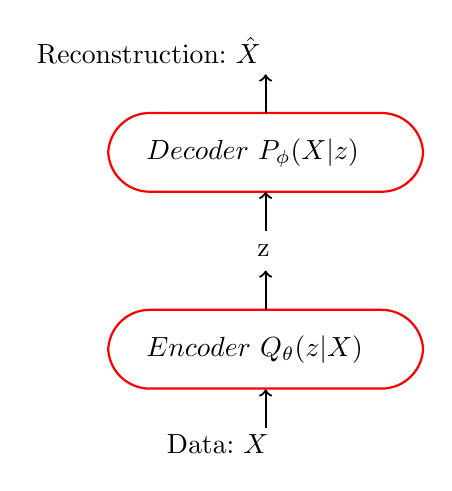
\begin{tikzpicture}

\visible<4->{
% text
\node[text width=0.007cm] at (8.40,5.75) {z};
\node[text width=0.007cm] at (7.25,3.3) {Data:~$X$};

\node[text width=0.01cm] at (6.99,4.5){$Encoder\ Q_\theta(z|X)$};

%circular rectangle
\draw[red!100,thick,solid,rounded corners=15pt] (6.5,4) rectangle (10.5,5);

%lines
\draw[thick,->] (8.5,3.5) -- (8.5,3.99);

\draw[thick,->] (8.5,5) -- (8.5,5.5);

}

\visible<5->{
	\node[text width=0.01cm] at (5.6,8.3) {Reconstruction:$\ \hat{X}$};
	\node[text width=0.01cm] at (6.99,6.99){$Decoder\ P_\phi(X|z)$};
	
	%circular rectangle
	\draw[red!100,thick,solid,rounded corners=15pt] (6.5,6.5) rectangle (10.5,7.5);
	
	%lines
	\draw[thick,->] (8.5,6) -- (8.5,6.5);
	
	\draw[thick,->] (8.5,7.5) -- (8.5,7.99);
	
}


\end{tikzpicture}
\end{center}

			\onslide<4->{$\theta$: the parameters of the encoder neural network}
			\onslide<5->{\\$\phi$: the parameters of the decoder neural network}
		\end{overlayarea}
		\column{0.6\textwidth}
		\begin{overlayarea}{\textwidth}{\textheight}
			\begin{itemize}\justifying
				\item<1-> We now return to our goals
				\item<2-> \textbf{Goal 1:} Learn a distribution over the latent variables ($Q(z|X)$)
				\item<3-> \textbf{Goal 2:} Learn a distribution over the visible variables ($P(X|z)$)
				\item<4-> VAEs use a neural network based encoder for Goal 1
				\item<5-> and a neural network based decoder for Goal 2
				\item<6-> We will look at the encoder first
%				\item<6-> Suppose we assume a certain form for the distribution $P(z|X)$ 
%				\item<7-> For example, let us assume that $P(z|X)$ is a Normal distribution 
%				\item<8-> In RBMs, we had assumed a certain structure (independencies) for the joint distribution whereas here we are assuming a certain family form for the distribution $P(z|X)$ 
			\end{itemize}
		\end{overlayarea}
	\end{columns}
\end{frame}


\begin{frame}
	\begin{columns}
		\column{0.42\textwidth}
		\begin{overlayarea}{\textwidth}{\textheight}
			\vspace{3pt}
			\only<1-4>{\input{modules/Module2/tikz_images/encoder_nn.tex}}
			\only<5->{\tikzstyle{input_neuron}=[circle,draw=red!50,fill=red!10,thick,minimum size=6mm]
\tikzstyle{hidden_neuron}=[circle,draw=blue!50,fill=cyan!10,thick,minimum size=6mm]
\tikzstyle{output_neuron}=[circle,draw=green!50,fill=green!10,thick,minimum size=6mm]

\tikzstyle{input}=[circle,draw=black!50,fill=black!20,thick,minimum size=6mm]

\begin{center}
\scalebox{0.7}{
\begin{tikzpicture}

\node [input_neuron] (neuron01) at (6.5,4.5) {};
\node [input_neuron] (neuron02) at (7.5,4.5){};
\node [input_neuron] (neuron03) at (8.5,4.5) {};
\node [input_neuron] (neuron04) at (9.5,4.5) {};
\node [input_neuron] (neuron05) at (10.5,4.5) {};
\node [hidden_neuron] (neuron51) at (6.5,6) {} ;
\node [hidden_neuron] (neuron52) at (7.5,6)  {};
\node [hidden_neuron] (neuron53) at (9.5,6)  {};
\node [hidden_neuron] (neuron54) at (10.5,6)  {};

\node [input_neuron] (neuron11) at (6.5,11)  {};
\node [input_neuron] (neuron12) at (7.5,11)  {};
\node [input_neuron] (neuron13) at (8.5,11)  {};
\node [input_neuron] (neuron14) at (9.5,11)  {};
\node [input_neuron] (neuron15) at (10.5,11)  {};

\node [ellipse,draw=red!50,fill=red!10,thick] (neuron16) at (8.5,8)  {Sample};

\node [] (neuron17) at (8.3,8.6)  {$z$};

\node[text width=0.01cm] at (8.3,3.3) {$\mathbf{X_i}$};
% \node[text width=0.007cm] at (7.7,5.25) {$\theta$};
\node[text width=0.007cm] at (11.2,4.5) {$Q_\theta(z|X)$};
\node[text width=0.01cm] at (11.2,6) {$\Sigma$};
\node[text width=0.01cm] at (5.6,6) {$\mu$};
% \node[text width=0.01cm] at (10.7,6) {$\mathbf{z}$};
% \node[text width=0.007cm] at (7.7,6.75) {$W^*$};
\node[text width=0.007cm] at (11.2,11) {$P_\phi(X|z)$};
\node[text width=0.01cm] at (8.3,12.2) {$\mathbf{\hat{X}_i}$};

\draw[red!100,thick,solid,rounded corners=15pt] (6,4) rectangle (11,5);
% \draw[red!100,thick,solid,rounded corners=15pt] (6.5,5.5) rectangle (10.5,6.5);
\draw[red!100,thick,solid,rounded corners=15pt] (6,5.5) rectangle (8.2,6.5);
\draw[red!100,thick,solid,rounded corners=15pt] (8.8,5.5) rectangle (11,6.5);
\draw[red!100,thick,solid,rounded corners=15pt] (6,10.5) rectangle (11,11.5);


\draw[thick,->] (8.5,3.5) -- (8.5,4);

\draw[thick,->] (8.5,5) -- (7.2,5.5);

\draw[thick,->] (8.5,5) -- (9.8,5.5);

\draw[thick,->] (7.2,6.5) -- (8.5,7.55);

\draw[thick,->] (9.8,6.5) -- (8.5,7.55);

\draw[thick,->] (8.5,8.45) -- (8.5,10.5);

\draw[thick,->] (8.5,11.5) -- (8.5,12);

\end{tikzpicture}}
\end{center}
}
			\onslide<5->{$X \in \mathbb{R}^n$, $\mu \in \mathbb{R}^m$ and $\Sigma \in \mathbb{R}^{m \times m}$}
		\end{overlayarea}
		\column{0.58\textwidth}
		\begin{overlayarea}{\textwidth}{\textheight}
			\begin{itemize}\justifying
%				\item<1-> Now given the assumption that $P(z|X)$ is a Normal distribution can you think of adapting the autoencoder architecture to learn the distribution $P(z|X)$ instead of learning $z$
				\item<1-> \textbf{Encoder:} What do we mean when we say we want to learn a distribution? \pause We mean that we want to learn the parameters of the distribution
				\item<3-> But what are the parameters of $Q(z|X)$? \onslide<4->{Well it depends on our modeling assumption!}
				\item<5-> In VAEs we assume that the latent variables come from a standard normal distribution $\mathcal{N}(0,I)$ and the job of the encoder is to then predict the parameters of this distribution
				%\item<5-> If $x \in R^n$ then $\mu \in R^n$ and $\sigma \in R^{n \times n}$
				%(on LHS figure now show how encoder predicts \Mu and \Sigma)
%				\item<3-> What are the parameters of a Normal Distribution? Mean ($\mu$) and Variance ($\sigma$)
%				\item<4-> So now what would you want the embedding generated by the encoder to represent ?
%				\item<5-> Well, we could design the encoder to predict the mean and variance of $P(z|X)$
			\end{itemize}
		\end{overlayarea}
	\end{columns}
\end{frame}

\begin{frame}
\begin{columns}
	\column{0.4\textwidth}
	\begin{overlayarea}{\textwidth}{\textheight}
		%\input{modules/Module2/tikz_images/autoencoder.tex}
   \tikzstyle{input_neuron}=[circle,draw=red!50,fill=red!10,thick,minimum size=6mm]
\tikzstyle{hidden_neuron}=[circle,draw=blue!50,fill=cyan!10,thick,minimum size=6mm]
\tikzstyle{output_neuron}=[circle,draw=green!50,fill=green!10,thick,minimum size=6mm]

\tikzstyle{input}=[circle,draw=black!50,fill=black!20,thick,minimum size=6mm]

\begin{center}
\scalebox{0.7}{
\begin{tikzpicture}

\node [input_neuron] (neuron01) at (6.5,4.5) {};
\node [input_neuron] (neuron02) at (7.5,4.5){};
\node [input_neuron] (neuron03) at (8.5,4.5) {};
\node [input_neuron] (neuron04) at (9.5,4.5) {};
\node [input_neuron] (neuron05) at (10.5,4.5) {};
\node [hidden_neuron] (neuron51) at (6.5,6) {} ;
\node [hidden_neuron] (neuron52) at (7.5,6)  {};
\node [hidden_neuron] (neuron53) at (9.5,6)  {};
\node [hidden_neuron] (neuron54) at (10.5,6)  {};

\node [input_neuron] (neuron11) at (6.5,11)  {};
\node [input_neuron] (neuron12) at (7.5,11)  {};
\node [input_neuron] (neuron13) at (8.5,11)  {};
\node [input_neuron] (neuron14) at (9.5,11)  {};
\node [input_neuron] (neuron15) at (10.5,11)  {};

\node [ellipse,draw=red!50,fill=red!10,thick] (neuron16) at (8.5,8)  {Sample};

\node [] (neuron17) at (8.3,8.6)  {$z$};

\node[text width=0.01cm] at (8.3,3.3) {$\mathbf{X_i}$};
% \node[text width=0.007cm] at (7.7,5.25) {$\theta$};
\node[text width=0.007cm] at (11.2,4.5) {$Q_\theta(z|X)$};
\node[text width=0.01cm] at (11.2,6) {$\Sigma$};
\node[text width=0.01cm] at (5.6,6) {$\mu$};
% \node[text width=0.01cm] at (10.7,6) {$\mathbf{z}$};
% \node[text width=0.007cm] at (7.7,6.75) {$W^*$};
\node[text width=0.007cm] at (11.2,11) {$P_\phi(X|z)$};
\node[text width=0.01cm] at (8.3,12.2) {$\mathbf{\hat{X}_i}$};

\draw[red!100,thick,solid,rounded corners=15pt] (6,4) rectangle (11,5);
% \draw[red!100,thick,solid,rounded corners=15pt] (6.5,5.5) rectangle (10.5,6.5);
\draw[red!100,thick,solid,rounded corners=15pt] (6,5.5) rectangle (8.2,6.5);
\draw[red!100,thick,solid,rounded corners=15pt] (8.8,5.5) rectangle (11,6.5);
\draw[red!100,thick,solid,rounded corners=15pt] (6,10.5) rectangle (11,11.5);


\draw[thick,->] (8.5,3.5) -- (8.5,4);

\draw[thick,->] (8.5,5) -- (7.2,5.5);

\draw[thick,->] (8.5,5) -- (9.8,5.5);

\draw[thick,->] (7.2,6.5) -- (8.5,7.55);

\draw[thick,->] (9.8,6.5) -- (8.5,7.55);

\draw[thick,->] (8.5,8.45) -- (8.5,10.5);

\draw[thick,->] (8.5,11.5) -- (8.5,12);

\end{tikzpicture}}
\end{center}

	\end{overlayarea}
	\column{0.6\textwidth}
	\begin{overlayarea}{\textwidth}{\textheight}
		\begin{itemize}\justifying
			\item<1-> Now what about the decoder?
			\item<2-> The job of the decoder is to predict a probability distribution over $X : P(X|z)$
			\item<3-> Once again we will assume a certain form for this distribution
			\item<4-> For example, if we want to predict 28 x 28 pixels and each pixel belongs to $\mathbb{R}$ (\textit{i.e.}, $X \in \mathbb{R}^{784}$) then what would be a suitable family for $P(X|z)$?
			\item<5-> We could assume that $P (X|z)$ is a Gaussian distribution with unit variance
			\item<6-> The job of the decoder $f$ would then be to predict the mean of this distribution as $f_\phi(z)$
		\end{itemize}
	\end{overlayarea}
\end{columns}
\end{frame}

\begin{frame}
\begin{columns}
	\column{0.4\textwidth}
	\begin{overlayarea}{\textwidth}{\textheight}
		%\input{modules/Module2/tikz_images/autoencoder.tex}
   \tikzstyle{input_neuron}=[circle,draw=red!50,fill=red!10,thick,minimum size=6mm]
\tikzstyle{hidden_neuron}=[circle,draw=blue!50,fill=cyan!10,thick,minimum size=6mm]
\tikzstyle{output_neuron}=[circle,draw=green!50,fill=green!10,thick,minimum size=6mm]

\tikzstyle{input}=[circle,draw=black!50,fill=black!20,thick,minimum size=6mm]

\begin{center}
\scalebox{0.7}{
\begin{tikzpicture}

\node [input_neuron] (neuron01) at (6.5,4.5) {};
\node [input_neuron] (neuron02) at (7.5,4.5){};
\node [input_neuron] (neuron03) at (8.5,4.5) {};
\node [input_neuron] (neuron04) at (9.5,4.5) {};
\node [input_neuron] (neuron05) at (10.5,4.5) {};
\node [hidden_neuron] (neuron51) at (6.5,6) {} ;
\node [hidden_neuron] (neuron52) at (7.5,6)  {};
\node [hidden_neuron] (neuron53) at (9.5,6)  {};
\node [hidden_neuron] (neuron54) at (10.5,6)  {};

\node [input_neuron] (neuron11) at (6.5,11)  {};
\node [input_neuron] (neuron12) at (7.5,11)  {};
\node [input_neuron] (neuron13) at (8.5,11)  {};
\node [input_neuron] (neuron14) at (9.5,11)  {};
\node [input_neuron] (neuron15) at (10.5,11)  {};

\node [ellipse,draw=red!50,fill=red!10,thick] (neuron16) at (8.5,8)  {Sample};

\node [] (neuron17) at (8.3,8.6)  {$z$};

\node[text width=0.01cm] at (8.3,3.3) {$\mathbf{X_i}$};
% \node[text width=0.007cm] at (7.7,5.25) {$\theta$};
\node[text width=0.007cm] at (11.2,4.5) {$Q_\theta(z|X)$};
\node[text width=0.01cm] at (11.2,6) {$\Sigma$};
\node[text width=0.01cm] at (5.6,6) {$\mu$};
% \node[text width=0.01cm] at (10.7,6) {$\mathbf{z}$};
% \node[text width=0.007cm] at (7.7,6.75) {$W^*$};
\node[text width=0.007cm] at (11.2,11) {$P_\phi(X|z)$};
\node[text width=0.01cm] at (8.3,12.2) {$\mathbf{\hat{X}_i}$};

\draw[red!100,thick,solid,rounded corners=15pt] (6,4) rectangle (11,5);
% \draw[red!100,thick,solid,rounded corners=15pt] (6.5,5.5) rectangle (10.5,6.5);
\draw[red!100,thick,solid,rounded corners=15pt] (6,5.5) rectangle (8.2,6.5);
\draw[red!100,thick,solid,rounded corners=15pt] (8.8,5.5) rectangle (11,6.5);
\draw[red!100,thick,solid,rounded corners=15pt] (6,10.5) rectangle (11,11.5);


\draw[thick,->] (8.5,3.5) -- (8.5,4);

\draw[thick,->] (8.5,5) -- (7.2,5.5);

\draw[thick,->] (8.5,5) -- (9.8,5.5);

\draw[thick,->] (7.2,6.5) -- (8.5,7.55);

\draw[thick,->] (9.8,6.5) -- (8.5,7.55);

\draw[thick,->] (8.5,8.45) -- (8.5,10.5);

\draw[thick,->] (8.5,11.5) -- (8.5,12);

\end{tikzpicture}}
\end{center}

	\end{overlayarea}
	\column{0.6\textwidth}
	\begin{overlayarea}{\textwidth}{\textheight}
		\begin{itemize}\justifying
			\item<1-> What would be the objective function of the decoder ?
			\item<2-> For any given training sample $x_i$ it should maximize $P(x_i)$ given by 
			\begin{align*}
				P(x_i) &= \int P(z)P(x_i|z) dz \\
				\onslide<3->{&=-\mathbb{E}_{z \sim Q_{\theta}(z|x_i)}[\log P_{\phi}(x_i|z)]}
			\end{align*}
			\item<4-> (As usual we take log for numerical stability)
		\end{itemize}
	\end{overlayarea}
\end{columns}
\end{frame}

\begin{frame}
\begin{columns}
	\column{0.4\textwidth}
	\begin{overlayarea}{\textwidth}{\textheight}
		%\input{modules/Module2/tikz_images/autoencoder.tex}	
	   \tikzstyle{input_neuron}=[circle,draw=red!50,fill=red!10,thick,minimum size=6mm]
\tikzstyle{hidden_neuron}=[circle,draw=blue!50,fill=cyan!10,thick,minimum size=6mm]
\tikzstyle{output_neuron}=[circle,draw=green!50,fill=green!10,thick,minimum size=6mm]

\tikzstyle{input}=[circle,draw=black!50,fill=black!20,thick,minimum size=6mm]

\begin{center}
\scalebox{0.7}{
\begin{tikzpicture}

\node [input_neuron] (neuron01) at (6.5,4.5) {};
\node [input_neuron] (neuron02) at (7.5,4.5){};
\node [input_neuron] (neuron03) at (8.5,4.5) {};
\node [input_neuron] (neuron04) at (9.5,4.5) {};
\node [input_neuron] (neuron05) at (10.5,4.5) {};
\node [hidden_neuron] (neuron51) at (6.5,6) {} ;
\node [hidden_neuron] (neuron52) at (7.5,6)  {};
\node [hidden_neuron] (neuron53) at (9.5,6)  {};
\node [hidden_neuron] (neuron54) at (10.5,6)  {};

\node [input_neuron] (neuron11) at (6.5,11)  {};
\node [input_neuron] (neuron12) at (7.5,11)  {};
\node [input_neuron] (neuron13) at (8.5,11)  {};
\node [input_neuron] (neuron14) at (9.5,11)  {};
\node [input_neuron] (neuron15) at (10.5,11)  {};

\node [ellipse,draw=red!50,fill=red!10,thick] (neuron16) at (8.5,8)  {Sample};

\node [] (neuron17) at (8.3,8.6)  {$z$};

\node[text width=0.01cm] at (8.3,3.3) {$\mathbf{X_i}$};
% \node[text width=0.007cm] at (7.7,5.25) {$\theta$};
\node[text width=0.007cm] at (11.2,4.5) {$Q_\theta(z|X)$};
\node[text width=0.01cm] at (11.2,6) {$\Sigma$};
\node[text width=0.01cm] at (5.6,6) {$\mu$};
% \node[text width=0.01cm] at (10.7,6) {$\mathbf{z}$};
% \node[text width=0.007cm] at (7.7,6.75) {$W^*$};
\node[text width=0.007cm] at (11.2,11) {$P_\phi(X|z)$};
\node[text width=0.01cm] at (8.3,12.2) {$\mathbf{\hat{X}_i}$};

\draw[red!100,thick,solid,rounded corners=15pt] (6,4) rectangle (11,5);
% \draw[red!100,thick,solid,rounded corners=15pt] (6.5,5.5) rectangle (10.5,6.5);
\draw[red!100,thick,solid,rounded corners=15pt] (6,5.5) rectangle (8.2,6.5);
\draw[red!100,thick,solid,rounded corners=15pt] (8.8,5.5) rectangle (11,6.5);
\draw[red!100,thick,solid,rounded corners=15pt] (6,10.5) rectangle (11,11.5);


\draw[thick,->] (8.5,3.5) -- (8.5,4);

\draw[thick,->] (8.5,5) -- (7.2,5.5);

\draw[thick,->] (8.5,5) -- (9.8,5.5);

\draw[thick,->] (7.2,6.5) -- (8.5,7.55);

\draw[thick,->] (9.8,6.5) -- (8.5,7.55);

\draw[thick,->] (8.5,8.45) -- (8.5,10.5);

\draw[thick,->] (8.5,11.5) -- (8.5,12);

\end{tikzpicture}}
\end{center}

		\vspace{-0.7cm}
		\begin{itemize}\justifying
			\item<5-> KL divergence captures the difference (or distance) between 2 distributions
		\end{itemize}
	\end{overlayarea}
	\column{0.6\textwidth}
	\begin{overlayarea}{\textwidth}{\textheight}
		\begin{itemize}\justifying
			\item<1-> This is the loss function for one data point $(l_i(\theta))$ and we will just sum over all the data points to get the total loss $\mathscr{L(\theta)}$
			\vspace{-0.8em}
			\begin{align*}
				\mathscr{L(\theta)}=\sum_{i=1}^ml_i(\theta)
			\end{align*}
			\vspace{-0.9em}
			\item<2-> In addition, we also want a constraint on the distribution over the latent variables 
			\item<3-> Specifically, we had assumed $P(z)$ to be $\mathcal{N}(0, I)$ and we want $Q(z|X)$ to be as close to $P(z)$ as possible
			\item<4-> Thus, we will modify the loss function such that 
			\begin{align*}
				l_i(\theta,\phi)=-\mathbb{E}_{z \sim Q_{\theta}(z|x_i)}& [\log P_{\phi}(x_i|z)] \\
				+ KL(&Q_{\theta}(z|x_i)||P(z))
			\end{align*}
		\end{itemize}
	\end{overlayarea}
\end{columns}
\end{frame}

\begin{frame}
\begin{columns}
	\column{0.4\textwidth}
	\begin{overlayarea}{\textwidth}{\textheight}
		%\input{modules/Module2/tikz_images/autoencoder.tex}
	    \tikzstyle{input_neuron}=[circle,draw=red!50,fill=red!10,thick,minimum size=6mm]
\tikzstyle{hidden_neuron}=[circle,draw=blue!50,fill=cyan!10,thick,minimum size=6mm]
\tikzstyle{output_neuron}=[circle,draw=green!50,fill=green!10,thick,minimum size=6mm]

\tikzstyle{input}=[circle,draw=black!50,fill=black!20,thick,minimum size=6mm]

\begin{center}
\scalebox{0.7}{
\begin{tikzpicture}

\node [input_neuron] (neuron01) at (6.5,4.5) {};
\node [input_neuron] (neuron02) at (7.5,4.5){};
\node [input_neuron] (neuron03) at (8.5,4.5) {};
\node [input_neuron] (neuron04) at (9.5,4.5) {};
\node [input_neuron] (neuron05) at (10.5,4.5) {};
\node [hidden_neuron] (neuron51) at (6.5,6) {} ;
\node [hidden_neuron] (neuron52) at (7.5,6)  {};
\node [hidden_neuron] (neuron53) at (9.5,6)  {};
\node [hidden_neuron] (neuron54) at (10.5,6)  {};

\node [input_neuron] (neuron11) at (6.5,11)  {};
\node [input_neuron] (neuron12) at (7.5,11)  {};
\node [input_neuron] (neuron13) at (8.5,11)  {};
\node [input_neuron] (neuron14) at (9.5,11)  {};
\node [input_neuron] (neuron15) at (10.5,11)  {};

\node [ellipse,draw=red!50,fill=red!10,thick] (neuron16) at (8.5,8)  {Sample};

\node [] (neuron17) at (8.3,8.6)  {$z$};

\node[text width=0.01cm] at (8.3,3.3) {$\mathbf{X_i}$};
% \node[text width=0.007cm] at (7.7,5.25) {$\theta$};
\node[text width=0.007cm] at (11.2,4.5) {$Q_\theta(z|X)$};
\node[text width=0.01cm] at (11.2,6) {$\Sigma$};
\node[text width=0.01cm] at (5.6,6) {$\mu$};
% \node[text width=0.01cm] at (10.7,6) {$\mathbf{z}$};
% \node[text width=0.007cm] at (7.7,6.75) {$W^*$};
\node[text width=0.007cm] at (11.2,11) {$P_\phi(X|z)$};
\node[text width=0.01cm] at (8.3,12.2) {$\mathbf{\hat{X}_i}$};

\draw[red!100,thick,solid,rounded corners=15pt] (6,4) rectangle (11,5);
% \draw[red!100,thick,solid,rounded corners=15pt] (6.5,5.5) rectangle (10.5,6.5);
\draw[red!100,thick,solid,rounded corners=15pt] (6,5.5) rectangle (8.2,6.5);
\draw[red!100,thick,solid,rounded corners=15pt] (8.8,5.5) rectangle (11,6.5);
\draw[red!100,thick,solid,rounded corners=15pt] (6,10.5) rectangle (11,11.5);


\draw[thick,->] (8.5,3.5) -- (8.5,4);

\draw[thick,->] (8.5,5) -- (7.2,5.5);

\draw[thick,->] (8.5,5) -- (9.8,5.5);

\draw[thick,->] (7.2,6.5) -- (8.5,7.55);

\draw[thick,->] (9.8,6.5) -- (8.5,7.55);

\draw[thick,->] (8.5,8.45) -- (8.5,10.5);

\draw[thick,->] (8.5,11.5) -- (8.5,12);

\end{tikzpicture}}
\end{center}

		\vspace{-0.7cm}
		\begin{align*}
		l_i(\theta,\phi)=-\mathbb{E}_{z \sim Q_{\theta}(z|x_i)}& [\log P_{\phi}(x_i|z)] \\
		+ KL(&Q_{\theta}(z|x_i)||P(z))
		\end{align*}
		%\vspace{-2.5em}
%		\begin{itemize}\justifying
%			\item<6-> But why do we choose a normal distribution? Isn't it too simplistic to assume that $z$ follows a normal distribution
%		\end{itemize}
	\end{overlayarea}
	\column{0.6\textwidth}
	\begin{overlayarea}{\textwidth}{\textheight}
		\begin{itemize}\justifying \footnotesize
			\item<1-> The second term in the loss function can actually be thought of as a regularizer
			\item<2-> It ensures that the encoder does not cheat by mapping each $x_i$ to a different point (a normal distribution with very low variance) in the Euclidean space 
			\item<3-> In other words, in the absence of the regularizer the encoder can learn a unique mapping for each $x_i$ and the decoder can then decode from this unique mapping
			\item<4-> Even with high variance in samples from the distribution, we want the decoder to be able to reconstruct the original data very well (motivation similar to the adding noise)
			\item<5-> To summarize, for each data point we predict a distribution such that, with high probability a sample from this distribution should be able to reconstruct the original data point
			\item<6-> But why do we choose a normal distribution? Isn't it too simplistic to assume that $z$ follows a normal distribution
		\end{itemize}
	\end{overlayarea}
\end{columns}
\end{frame}

%slide 13
%\begin{frame}
%	\begin{columns}
%		\column{0.4\textwidth}
%		\begin{overlayarea}{\textwidth}{\textheight}
%			\vspace{3pt}
%			\input{modules/Module1/tikz_images/autoencoder.tex}
%		\end{overlayarea}
%		\column{0.6\textwidth}
%		\begin{overlayarea}{\textwidth}{\textheight}
%			\begin{itemize}\justifying
%				\item<1-> But how will we train the encoder ?
%				\item<2-> What is the loss function that we will use ?
%				\item<3-> More specifically, how will we ensure that the $\mu$ and $\sigma$ that the encoder produces are the true $\mu$ and $\sigma$ of $P(z|X)$
%				\item<4-> We don't even know what the true $\mu$ and $\sigma$ are then how to we guide/train the model to produce these $\mu$ and $\sigma$
%				\item<5-> \textbf{Spoiler Alert:} We will be making some assumptions but to see why these assumptions make sense we will first revisit the concept of latent variables
%			\end{itemize}
%		\end{overlayarea}
%	\end{columns}
%\end{frame}

%slide 14
%\begin{frame}
%	\begin{columns}
%		\column{0.4\textwidth}
%		\begin{overlayarea}{\textwidth}{\textheight}
%			% LHS: show some images of MNIST
%			\vspace{3pt}
%			\begin{figure}
%				\centering
%				\includegraphics[scale=0.3]{images/mnist.png}
%			\end{figure}
%		\end{overlayarea}
%		\column{0.6\textwidth}
%		\begin{overlayarea}{\textwidth}{\textheight}
%			\begin{itemize}\justifying
%				\item<1-> Consider images of handwritten digits where visible random variables are the pixels of the image
%				\item<2-> And we can think of several latent variables ($z$): the digit, size, angle, thickness, position and so on
%				\item<3-> It is reasonable to argue that once we select a $z$, the image is actually a deterministic function of $z$
%				\item<4-> For example, once the digit, size, angle thickness, position, \textit{etc.} are fixed we know exactly what the image should look like
%				\item<5-> Of course, we are assuming that we have enough latent variables to capture all characteristics of handwritten digits 
%			\end{itemize}
%		\end{overlayarea}
%	\end{columns}
%\end{frame}

%slide 15
%\begin{frame}
%	\begin{columns}
%		\column{0.4\textwidth}
%		\begin{overlayarea}{\textwidth}{\textheight}
%			\vspace{3pt}
%			\begin{figure}
%				\centering
%				\includegraphics[scale=0.3]{images/mnist.png}
%			\end{figure}
%		\end{overlayarea}
%		\column{0.6\textwidth}
%		\begin{overlayarea}{\textwidth}{\textheight}
%			\begin{itemize}\justifying
%				\item<1-> Of course, even though deterministic, the image (or visible variables) may still be a complex function of the hidden variables $z$
%				\item<2-> In others words, $X = f (z; \theta)$ where $z$ is a complex function and $\theta$ are the parameters of this complex function
%				\item<3-> Can you think of how you could model such a complex function ? 
%				\item<4-> Well, we could use a deep neural network which is good at approximating arbitrary complex functions (recall Universal Approximation Theorem)
%				\item<5-> With this intuition, we will now look at the full picture and discuss the objective function
%			\end{itemize}
%		\end{overlayarea}
%	\end{columns}
%\end{frame}

%slide 16
%\begin{frame}
%	\begin{columns}
%		\column{0.4\textwidth}
%		\begin{overlayarea}{\textwidth}{\textheight}
%			% LHS: Show the VAE diagram the VAE tutorial but one step at a time synced with the bullets
%			\vspace{4mm}
%			\begin{tikzpicture}
%				\node[inner sep=0pt] (encoder) at (0,0) {\includegraphics[scale=0.15]{images/vae_encoder.png}};
%				\onslide<3->{\node[inner sep=0pt] (sample) at (0,2) {\includegraphics[scale=0.15]{images/vae_sample.png}};
%				\draw[->,thick] (encoder.north) -- (sample.south);
%				}
%				\onslide<4->{\node[inner sep=0pt] (decoder) at (0,4) {\includegraphics[scale=0.15]{images/vae_decoder.png}};
%				\draw[->,thick] (sample.north) -- (decoder.south);
%				}
%			\end{tikzpicture}
%		\end{overlayarea}
%		\column{0.6\textwidth}
%		\begin{overlayarea}{\textwidth}{\textheight}
%			\begin{itemize}\justifying
%				\item<1-> First, the task of the encoder is to predict the parameters $(\mu, \sigma)$ of $P(z|X)$
%				\item<2-> So given a training sample $X$, the encoder will first produce $\mu(X), \sigma(X)$
%				\item<3-> We will now sample a hidden variable $z$ from the distribution $N(\mu(X), \sigma(X))$
%				\item<4-> The job of the decoder is to then reconstruct X from this sampled $z$
%			\end{itemize}
%		\end{overlayarea}
%	\end{columns}
%\end{frame}

%slide 17
%\begin{frame}
%	\begin{columns}
%		\column{0.4\textwidth}
%		\begin{overlayarea}{\textwidth}{\textheight}
%			\vspace{4mm}
%			\begin{tikzpicture}
%				\node[inner sep=0pt] (encoder) at (0,0) {\includegraphics[scale=0.15]{images/vae_encoder.png}};
%				\node[inner sep=0pt] (sample) at (0,2) {\includegraphics[scale=0.15]{images/vae_sample.png}};
%				\draw[->,thick] (encoder.north) -- (sample.south);
%				\node[inner sep=0pt] (decoder) at (0,4) {\includegraphics[scale=0.15]{images/vae_decoder.png}};
%				\draw[->,thick] (sample.north) -- (decoder.south);
%			\end{tikzpicture}
%		\end{overlayarea}
%		\column{0.6\textwidth}
%		\begin{overlayarea}{\textwidth}{\textheight}
%			\begin{itemize}\justifying
%				\item<1-> Given this setup what should be the loss function for the decoder
%				\begin{align*}
%					||X - f(z; \theta)||^2
%				\end{align*}
%				\item<2-> But what about the encoder? What kind of loss function would ensure $\mu$ and $\sigma$ that the encoder produces are the true $\mu$ and $\sigma$ of $P(z|X)$ ?
%				\item<3-> Well if we knew the true $P(z)$ then we could have minimized the KL divergence between $Q(z|X)$ and $P(z)$
%				\item<4-> But we don't know what $P(z)$ is so we will make an assumption that $P(z)$ is $N(0, I)$
%			\end{itemize}
%		\end{overlayarea}
%	\end{columns}
%\end{frame}


\begin{frame}
	\begin{columns}
		\column{0.4\textwidth}
		\begin{overlayarea}{\textwidth}{\textheight}
			% LHS: SHow Figure 2 from tutorial
			\begin{figure}
				\centering
				\includegraphics[scale=0.2]{images/2d_dist.png}
			\end{figure}
			\vspace{-0.6cm}
			\begin{figure}
				\centering
				\includegraphics[scale=0.2]{images/2d_trans.png}
			\end{figure}
			\vspace{-0.6cm}
			\begin{align*}
				l_i(\theta,\phi)=-\mathbb{E}_{z \sim Q_{\theta}(z|x_i)}& [\log P_{\phi}(x_i|z)] \\
				+ KL(&Q_{\theta}(z|x_i)||P(z))
			\end{align*}
		\end{overlayarea}
		\column{0.6\textwidth}
		\begin{overlayarea}{\textwidth}{\textheight}
			\begin{itemize}\justifying
				\item<1-> Isn't it a very strong assumption that $P(z) \sim \mathcal{N}(0, I)$ ?
				\item<2-> For example, in the 2-dimensional case how can we be sure that $P(z)$ is a normal distribution and not any other distribution
				\item<3-> The key insight here is that any distribution in $d$ dimensions can be generated by the following steps
				\item<4-> Step 1: Start with a set of $d$ variables that are normally distributed (that's exactly what we are assuming for $P(z)$)
				\item<5-> Step 2: Mapping these variables through a sufficiently complex function (that's exactly what the first few layers of the decoder can do)
			\end{itemize}
		\end{overlayarea}
	\end{columns}
\end{frame}


\begin{frame}
	\begin{columns}
		\column{0.4\textwidth}
		\begin{overlayarea}{\textwidth}{\textheight}
			% LHS: SHow Figure 2 from tutorial
			\begin{figure}
				\centering
				\includegraphics[scale=0.2]{images/2d_dist.png}
			\end{figure}
			\vspace{-0.6cm}
			\begin{figure}
				\centering
				\includegraphics[scale=0.2]{images/2d_trans.png}
			\end{figure}
			\vspace{-0.6cm}
			\begin{align*}
				l_i(\theta,\phi)=-\mathbb{E}_{z \sim Q_{\theta}(z|x_i)}& [\log P_{\phi}(x_i|z)] \\
				+ KL(&Q_{\theta}(z|x_i)||P(z))
			\end{align*}
		\end{overlayarea}
		\column{0.6\textwidth}
		\begin{overlayarea}{\textwidth}{\textheight}
			\footnotesize{\begin{itemize}\justifying
				\item<1-> In particular, note that in the adjoining example if $z$ is 2-D and normally distributed then $f(z)$ is roughly ring shaped (giving us the distribution in the bottom figure)
				\vspace{-4mm}
				\begin{align*}
				f(z) = \frac{z}{10} + \frac{z}{||z||}
				\end{align*}
				\vspace{-6mm}
				\item<2-> A non-linear neural network, such as the one we use for the decoder, could learn a complex mapping from $z$ to $f_\phi(z)$ using its parameters $\phi$
%				\item<2-> In other words, 
%				\vspace{-4mm}
%				\begin{align*}
%				g(z) = \theta_1 z + \theta_2 z
%				\end{align*}
%				\vspace{-8mm}
				\item<3-> The initial layers of a non linear decoder could learn their weights such that the output is $f_\phi(z)$
				\item<4-> The above argument suggests that even if we start with normally distributed variables the initial layers of the decoder could learn a complex transformation of these variables say $f_\phi(z)$ if required
				\item<5-> The objective function of the decoder will ensure that an appropriate transformation of z is learnt to reconstruct $X$
			\end{itemize}}
		\end{overlayarea}
	\end{columns}
\end{frame}


%\begin{frame}
%	\begin{columns}
%		\column{0.4\textwidth}
%		\begin{overlayarea}{\textwidth}{\textheight}
%			\vspace{4mm}
%			\begin{tikzpicture}
%				\node[inner sep=0pt] (encoder) at (0,0) {\includegraphics[scale=0.15]{images/vae_encoder.png}};
%				\node[inner sep=0pt] (sample) at (0,2) {\includegraphics[scale=0.15]{images/vae_sample.png}};
%				\draw[->,thick] (encoder.north) -- (sample.south);
%				\node[inner sep=0pt] (decoder) at (0,4) {\includegraphics[scale=0.15]{images/vae_decoder.png}};
%				\draw[->,thick] (sample.north) -- (decoder.south);
%			\end{tikzpicture}
%		\end{overlayarea}
%		\column{0.6\textwidth}
%		\begin{overlayarea}{\textwidth}{\textheight}
%			\begin{itemize}\justifying
%				\item<1-> So now that we are convinced that it is okay to assume P(z) is N(0, I) then the objective function of the encoder is straightforward
%				\item<2-> We simply need to minimize $KL[N(\mu(X), \sigma(X)), N(0, I)]$
%				\item<3-> That completes the full picture and we will summarize the discussion on the next slide
%			\end{itemize}
%		\end{overlayarea}
%	\end{columns}
%\end{frame}


%\begin{frame}
%	\begin{columns}
%		\column{0.4\textwidth}
%		\begin{overlayarea}{\textwidth}{\textheight}
%			\vspace{4mm}
%			\begin{tikzpicture}
%				\node[inner sep=0pt] (encoder) at (0,0) {\includegraphics[scale=0.15]{images/vae_encoder.png}};
%				\node[inner sep=0pt] (sample) at (0,2) {\includegraphics[scale=0.15]{images/vae_sample.png}};
%				\draw[->,thick] (encoder.north) -- (sample.south);
%				\node[inner sep=0pt] (decoder) at (0,4) {\includegraphics[scale=0.15]{images/vae_decoder.png}};
%				\draw[->,thick] (sample.north) -- (decoder.south);
%			\end{tikzpicture}
%		\end{overlayarea}
%		\column{0.6\textwidth}
%		\begin{overlayarea}{\textwidth}{\textheight}
%			\begin{itemize}\justifying
%				\item<1-> Encoder: Generates the $\mu$ and $\sigma$ of $Q(z|X)$
%				\item<2-> Decoder: Samples from $Q(z|X)$ and reconstructs $X$
%				\item<3-> Encoder loss: 
%				\begin{align*}
%				min \hspace{3mm}KL[N(\mu(X), \Sigma(X)), N(0, I)]
%				\end{align*}
%				\item<4-> Decoder loss: 
%				\begin{align*}
%				min \hspace{3mm}||X - f(z; \theta)||^2
%				\end{align*}
%				\item<5-> There are still a few pieces missing and we will get back to them later
%			\end{itemize}
%		\end{overlayarea}
%	\end{columns}
%\end{frame}


%\begin{frame}
%	\begin{columns}
%		\column{0.4\textwidth}
%		\begin{overlayarea}{\textwidth}{\textheight}
%			\vspace{4mm}
%			\begin{tikzpicture}
%				\node[inner sep=0pt] (encoder) at (0,0) {\includegraphics[scale=0.15]{images/vae_encoder.png}};
%				\node[inner sep=0pt] (sample) at (0,2) {\includegraphics[scale=0.15]{images/vae_sample.png}};
%				\draw[->,thick] (encoder.north) -- (sample.south);
%				\node[inner sep=0pt] (decoder) at (0,4) {\includegraphics[scale=0.15]{images/vae_decoder.png}};
%				\draw[->,thick] (sample.north) -- (decoder.south);
%			\end{tikzpicture}
%		\end{overlayarea}
%		\column{0.6\textwidth}
%		\begin{overlayarea}{\textwidth}{\textheight}
%			\begin{itemize}\justifying
% 				\item<1-> This was a very simplistic (non-rigorous) introduction to VAEs
% 				\item<2-> We will now do a more rigorous discussion on the Math behind VAEs
%			\end{itemize}
%		\end{overlayarea}
%	\end{columns}
%\end{frame}

